\documentclass[12pt]{article}
%%% DOCUMENT FORMATTING %%%
\usepackage[margin=1in]{geometry}
\usepackage{enumitem}
\setlength{\parindent}{0pt}
\newcommand{\disp}{\displaystyle}

%%% HEADER %%%
\usepackage{fancyhdr}
\pagestyle{fancy}
\fancyhf{}
\lhead{MATH 1060}
\rhead{Vagnozzi}
\cfoot{\thepage}

%%% MATH NOTATION & SYMBOLS %%%
\usepackage{amssymb}
\usepackage{amsmath}
\newcommand{\R}{\mathbb{R}}
\newcommand{\N}{\mathbb{N}}
\newcommand{\Z}{\mathbb{Z}}
\newcommand{\lp}{\left(}
\newcommand{\rp}{\right)}
\newcommand{\ls}{\left[}
\newcommand{\rs}{\right]}
\newcommand{\lb}{\left\{}
\newcommand{\rb}{\right\}}
\newcommand{\arccot}{\text{arccot}}
\newcommand{\arccsc}{\text{arccsc}}
\newcommand{\arcsec}{\text{arcsec}} 

%%% TABLES %%%
\usepackage{colortbl}

%%% GRAPHS %%%
\usepackage{tikz}
\usepackage{pgfplots}
\pgfplotsset{compat=1.15}
\usepgfplotslibrary{fillbetween}
\usetikzlibrary{angles,quotes}

%%% ENVIRONMENTS %%%
\newcommand{\Example}{\paragraph{\Writinghand \hspace{0.1mm} Example.}}
\newcommand{\ExampleCont}{\paragraph{\Writinghand \hspace{0.1mm} Example (continued).}}
\newcommand{\boxenv}[2]{
	\fbox{
	\begin{minipage}{0.97\textwidth}
	\vspace{2mm}	
	\paragraph{#1} #2
	\vspace{2mm}
	\end{minipage}
	}}

%%% FUN THINGS %%%
\newcommand*\tc[1]{\tikz[baseline=(char.base)]{
            \node[shape=circle,draw,inner sep=2pt] (char) {#1};}}
\usepackage{marvosym}

%%% MISC %%%
\usepackage{hyperref}


\setcounter{page}{186}

\begin{document}
\section*{5.4: Applications of Integration}

\boxenv{Learning Objectives.}{Upon successful completion of Section 5.4, you will be able to\dots
		
	\begin{itemize}[leftmargin=6mm]
		\item Answer conceptual questions involving symmetry and average value of functions.
		\item Use symmetry to evaluate definite integrals.
		\item Find average value of functions over given intervals.
		\item Solve applications involving average value of functions.
		\item Solve problems involving the Mean Value Theorem for Integrals.
	\end{itemize}
	\vspace{-4mm}
}

\vspace{5mm}

\subsection*{Average of a Function}

Recall from previous courses that the \textbf{average} of a finite set $\mathcal{S}$ can be found by summing the values in the set and dividing by the number of values in the set.

$$\mathcal{S}=\lb 1,2,3,4,5 \rb \,\Longrightarrow\,\mathcal{S}_\text{avg}=\frac{1}{\vert\mathcal{S}\vert}\sum_{i=1}^5 s_i=\frac{1+2+3+4+5}{5}=3$$

\vspace{3mm}

How could we calculate the average of a \textit{function} $f$ (i.e.\ the average $y$-value) on a closed interval $[a,b]$?

\newpage

\boxenv{Definition.}{The \textbf{average value} of a continuous function $f$ on the interval $[a,b]$ is
\vspace{15mm}
}

\vspace{3mm}

\paragraph{Geometric Interpretation.} If $f>0$ on $[a,b]$, then $\overline{f}$ gives the height of a rectangle with base $b-a$ whose area matches the area under the curve.

\vspace{5mm}

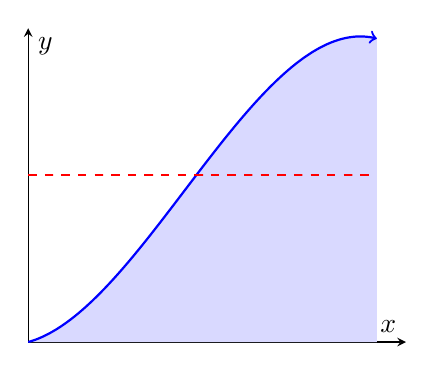
\begin{tikzpicture}[scale=0.7]
      \begin{axis}[
                    %minor tick num=2,
                    name path=f,
                	axis x line=middle,
                	axis y line=center,
                	xmax=130, xmin=0,
                	ymax=15.5, ymin=0,
                	xlabel=$x$,ylabel=$y$,
                	xtick={\empty},ytick={\empty}
                    ]
                    
                    \addplot[name path=f, smooth,color=blue,domain=0:120,samples=50,thick,->] {(	-0.000017183)*x^3 + (	0.00277282)*x^2 +	0.0396189*x};
    \path[name path=axis] (axis cs:0,0) -- (axis cs:120,0);
        
        \addplot[name path=g, smooth,color=red,domain=0:120,samples=50,thick,dashed] {8.264};

            \addplot+[blue!15] fill between[of=f and axis,soft clip={domain=0:120}];
            %\addplot+[red!15] fill between[of=g and axis,soft clip={domain=0:120}];

%                \node[label={[red]0:{$\bar{f}$}},inner sep=2pt] at (axis cs:120,8.264) {};


                \end{axis}
            \end{tikzpicture}
            
\vspace{5mm}

\Example Find the average value of $f(x)=\cos x$ on the interval $\ls 0,\frac{\pi}{4}\rs$.

\vspace{40mm}

\Example If $f$ is linear on $[a,b]$, show that $\overline{f}=f\lp\disp\frac{a+b}{2}\rp$. Use this result to find the average of $f(x)=8x-3$ on $[0,1]$.

\newpage

\Example If $f(x)=ax^2+1$, find $a\in\R$ so that $\overline{f}=\pi$ on $[-1,1]$.

\vspace{50mm}

\subsection*{Mean Value Theorem for Integrals}

In Section 4.2, we learned about the Mean Value Theorem for functions. We can extend this theorem to integrals now that we have the definition of the average value of a function.

\vspace{5mm}

\boxenv{Mean Value Theorem for Integrals (MVTI).}{Let $f$ be continuous on $[a,b]$. Then there exists a point $c\in(a,b)$ such that $f(x)=\overline{f}$.}

\vspace{5mm}

\Example Apply the MVTI to $f(x)=4-x^2$ on the interval $[-2,0]$.

\newpage

\subsection*{Integrating Functions with Symmetry}

A function is called \textbf{even} if it has $y$-axis symmetry.

\vspace{30mm}

A function is called \textbf{odd} if it has origin symmetry.

\vspace{30mm}

We can take advantage of symmetry to simplify integration.

\vspace{5mm}

\boxenv{Parity of $f$ and $F$.}{Suppose $F$ is an antiderivative of $f$. If $f$ is even, then $F$ is odd. Alternatively, if $f$ is odd, then $F$ is even.}

\vspace{5mm}

\boxenv{Even and Odd Integrands.}{Let $a>0$ and let $f$ be integrable on $[-a,a]$.
\begin{itemize}
\item If $f$ is even, then $\disp\int_{-a}^a f(x)\,dx=2\int_0^a f(x)\,dx$.
\item If $f$ is odd, then $\disp\int_{-a}^a f(x)\,dx=0$.
\end{itemize}
\vspace{-2mm}}

\vspace{30mm}

\boxenv{Remark.}{The sine function is odd while the cosine function is even.

$$\sin(-x)=-\sin x\hspace{20mm} \cos(-x)=\cos x$$

\vspace{-3mm}}

\newpage

\Example Evaluate the following definite integrals.
\begin{itemize}
	\item[\tc{1}] $\disp\int_{-\frac{\pi}{8}}^{\frac{\pi}{8}}\sin x\, dx$
	
	\vspace{20mm}
	
	\item[\tc{2}] $\disp\int_{-4}^4(4-x^2)\,dx$
\end{itemize}
\end{document}